\documentclass[10pt]{article}
\usepackage{parskip}
\usepackage[utf8]{inputenc}
\usepackage[left=2.00cm, right=2.00cm, top=2.00cm, bottom=2.00cm]{geometry}
\usepackage[spanish]{babel}
\usepackage{graphicx,subfig}
\usepackage{fancyhdr}
\usepackage{pgfplots}
\graphicspath{{Imagenes/}}
\usepackage{enumerate} 
\usepackage{multicol}
\usepackage{tabularx}
\usepackage{amssymb}
\usepackage{adjustbox}
\usepackage{amsmath}
\usepackage{cancel}
\begin{document}


\pagestyle{fancy}
\cfoot{}


%Cabeceras
\rhead{Superposición de Ondas.}
\lhead{}

%Portada
\begin{titlepage}
	\newgeometry{
		left=25mm,
		right=25mm,
		top=5mm,
		bottom=30mm,
		headheight = 0 mm
	}

	\begin{figure}[t]
		\subfloat{
\includegraphics[width=0.15\textwidth]{Logo_IPN}}
		\hspace{0.6\textwidth}
		\subfloat{
\includegraphics[width=0.22\textwidth]{LogoEsime}}
	\end{figure}

	\centering
	{\bfseries\Huge Instituto Politécnico Nacional. \par}
	\vspace{1cm}
	{\scshape\Large Ingeniería en Comunicaciones y Electrónica. \par}
	\vspace{0.3cm}
	{\scshape\Large Laboratorio de Electricidad y Magnetismo.  \par}
	\vspace{1cm}
	{\scshape\Huge - - ..- -.-. .... .- ... / - - - -. -.. .- ... .-.-. \par}
	\vspace{1cm}
	{\itshape\Large Superposición de Ondas \par}
	{\Large 2CM13\par}
	\vfill
	
	{\Large  \par}
	{\Large   \par}
	{\Large  \par}
	{\Large \par}
	{\Large   \par}
	{\Large \par}
	\vfill
	{\Large Octubre 2023. \par}

\end{titlepage}

\tableofcontents
\newpage
\begin{center}
	Hernández Huerta Jose Emilio, 
	Hernández Sanluis Danna Estefany,  
	Garduño Bejarano Nataly,
	Mojica Reyes Rogelio,
	Morlan Juárez Bruno Tonatiuh,  
	Santos Marañón María Renée.
\end{center}

\section{Resumen.}
Dentro de este reporte de laboratorio usted podrá observar y verificar el desarrollo mediante el cual se explica cómo es que mediante el uso del osciloscopio y un generador obtenemos las figuras o curvas de Lissajous, es decir una gráfica producida por determinadas frecuencias, lo anterior está basado en los términos manejados en clase. Las figuras de Lissajous son la combinación de dos movimientos armónicos, que dan lugar a interesantes figuras, que por lo general son simétricas. Podemos reproducir estas curvas en el osciloscopio, poniéndolo en posición X-Y, y aplicando dos señales de distinta o igual frecuencia y desfase. Aplicando dos sinusoides se pueden lograr miles de figuras.

\begin{multicols}{2}

\section{Objetivo.}

Adquirir un conocimiento integral sobre el fenómeno de interferencia y superposición de ondas, centrándose en cómo la combinación de dos o más ondas influye en la amplitud y fase resultantes, y cómo estas combinaciones pueden conducir a la interferencia constructiva o destructiva. Además, se busca dominar la capacidad de medir con precisión amplitudes, frecuencias, longitudes de onda y velocidades de propagación en situaciones de ondas superpuestas.



\section{Marco teórico.}
\subsection{ Definición de Ondas Magnéticas:} 
Las ondas magnéticas son perturbaciones en el campo magnético que se propagan a través del espacio. Estas ondas se generan mediante la variación de campos magnéticos en el tiempo, como ocurre en corrientes eléctricas alternas.
\subsection{Características de las Ondas Magnéticas:}
Frecuencia y Longitud de Onda: Al igual que las ondas electromagnéticas, las ondas magnéticas tienen una frecuencia y longitud de onda asociadas. La frecuencia determina la cantidad de oscilaciones por unidad de tiempo, mientras que la longitud de onda es la distancia entre dos puntos idénticos en la onda.
Velocidad de Propagación: La velocidad de propagación de las ondas magnéticas está relacionada con las propiedades magnéticas del medio a través del cual se propagan.
\subsection{Principio de Superposición:}
 La superposición de ondas magnéticas es un principio que establece que, cuando dos o más ondas magnéticas se encuentran en un punto en el espacio, la magnitud resultante del campo magnético es la suma algebraica de las magnitudes individuales de las ondas en ese punto. La superposición permite analizar sistemas complejos de ondas magnéticas al considerar la contribución de cada onda por separado y luego sumarlas vectorialmente.
 \subsection{Interferencia de Ondas Magnéticas: Interferencia Constructiva:} Ocurre cuando las crestas de dos ondas coinciden, aumentando la magnitud del campo magnético resultante. Interferencia Destructiva: Ocurre cuando una cresta coincide con una depresión, dando lugar a una reducción en la magnitud del campo magnético resultante.
 \subsection{Ejemplos Prácticos: Aplicaciones en Comunicaciones:} 
 La superposición de ondas magnéticas es esencial en tecnologías como la modulación de frecuencia (FM) y la modulación de amplitud (AM) utilizadas en la transmisión de señales de radio y televisión. Resonancia Magnética (RM): En medicina, la RM utiliza campos magnéticos para generar imágenes detalladas del interior del cuerpo, aprovechando los principios de superposición de ondas magnéticas.

\section{Experimento 1 - Generación de figuras Lissajous}
 \textbf{Procedimiento Experimental:}
 Para la generación de figuras Lissajous es necesario tener en cuenta que hablamos del uso de ondas superpuestas, y para lograr la visualización de las anteriores usamos como base dos generadores de señales, los cuales calibramos a ciertas frecuencias para sobreponerlas y proyectarlas a un osciloscopio (previamente antes calibrado, para focalizar las dos ondas en un solo plano y en una visión más general).
 Posteriormente procedimos a empezar a generar nuestras ondas y así cumplir con nuestro cometido, pero cabe aclarar que en todos los resultados nuestros valores en cuanto magnitud de frecuencia se trataban, no eres muy congruentes a pesar de que tratamos de que los valores fueran lo más apegados a lo teórico, las gráficas no resultaban en ninguna figura o señal aceptable para considerar que teníamos un resultado. Por lo que nuestra conclusión ante tal variación de parámetros se lo adjudicamos al equipo con el que trabajamos, ya sea por la des calibración que estos llevaban o por su tiempo anterior de uso. Una vez aclarado lo anterior presentaremos valores experimentales en su gran mayoría.
 Como nota extra nosotros usamos w (omega minúscula), como si fuera una frecuencia normal, pero nosotros al saber que hablamos de frecuencia angular, lo pusimos generalizar de la siguiente manera. \\ 
 \begin{center}
$\omega_{1}=\nu_{1}$\&$\omega_{2}=\nu_{2}$\\
 \end{center}
 

Por lo tanto, no tenemos problemas en usar las frecuencias de los generadores como frecuencias angulares.
A continuación, presentaremos los casos de cada fila que se presentan en la tabla 1 (Esta la presentaremos en el apartado de Resultados), como manejamos las frecuencias y una imagen de cada caso ya antes mencionado.
\textbf{Señal 1}\\
\begin{center}
   $ \frac{\omega_{1}}{\omega_{2}}=\frac{21.05 kHz }{21.05 kHz }$\\
\end{center}

Para el valor de las dos  generadores de señales establecimos el mismo valor (21.05), arrojando el siguiente dato Figura 1.\\

\begin{center}
	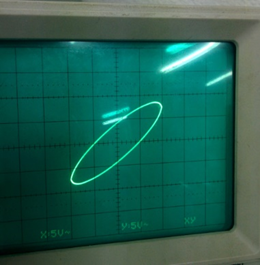
\includegraphics[width=4cm,height=5cm]{Imagenes/1.png}
	\captionof{figure}{Osciloscopio con el primer primer valor de la tabla.}
	\label{fig:1}
\end{center}
\textbf{Señal 2}\\
\begin{center}
    
$\frac{\omega_{1}}{2\omega_{2}}=\frac{10.15}{20.29}$\\
\end{center}
Para la segunda señal disminuimos la frecuencia del primer generador de señales a un valor de 10.15 kHz multiplicando por 2 para el valor del segundo generador obteniendo un valor de 20.29 kHz, arrogando una figura en el osciloscopio (Figura 2)\\
\begin{center}
	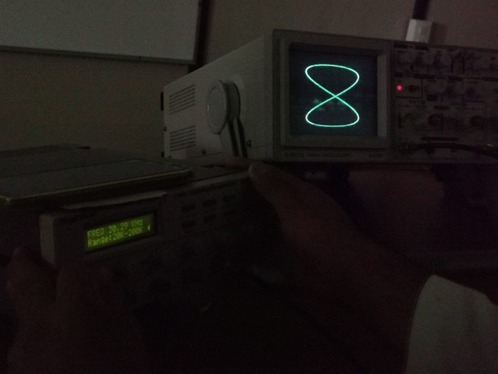
\includegraphics[width=4cm,height=5cm]{Imagenes/2.png}
	\captionof{figure}{Imagen del osciloscopio y del generador de señal con el valor de 20.29 kHz.}
	\label{fig:2}
\end{center}
\textbf{Señal 3}\\
\begin{center}
    
$\frac{2\omega_{1}}{\omega_{2}}=\frac{21.05}{10.03}$\\
\end{center}
En la 3ra señal se ocupó como un valor base de 10.03 que colocamos en el segundo generador de señales multiplicando su valor por 2 dando un valor de 20.06 kHz para el primer generador de 
señales, pero por errores de calibración y que se muestre así una imagen congruente, el valor lo establecimos como 21.05 kHz. (Figura 3)\\

\begin{center}
	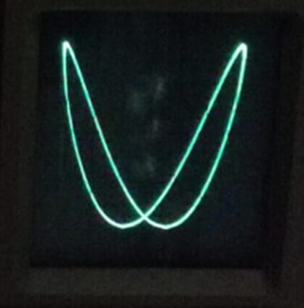
\includegraphics[width=4cm,height=5cm]{Imagenes/3.png}
	\captionof{figure}{Dibujo de una silla para montar.}
	\label{fig:3}
\end{center}
\textbf{Señal 4}\\
\begin{center}
    
$\frac{\omega_{1}}{3\omega_{2}}=\frac{5.113}{14.49}$\\
\end{center}
Para esta señal ocupamos una frecuencia inicial en el generador 1 de 5.113 y en el segundo generador agregamos un valor 3 veces mayor al del generador 1 que es 15 kHz, por errores de tabulación se estableció a un valor aproximado a 15 kHz que es 14.49 kHz. (Figura 4)\\
\begin{center}
	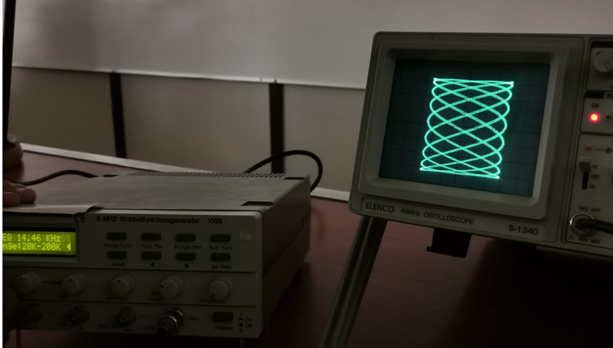
\includegraphics[width=4cm,height=5cm]{Imagenes/4.png}
	\captionof{figure}{Imagen arrojada por el osciloscopio.}
	\label{fig:4}
\end{center}

\textbf{Señal 5}\\
\begin{center}
    
$\frac{3\omega_{1}}{\omega_{2}}=\frac{15.30 kHz}{4.988 kHz}$\\
\end{center}
Para esta señal pusimos un valor determinado a 5 kHz para el generador 2, estableciendo asi en el primer generador 3 veces el valor del 2do, por lo que para el generador 1 tiene un valor de 15.30 kHz y en el 2 un valor de 4.988 kHz. (Figura 5)\\
\begin{center}
	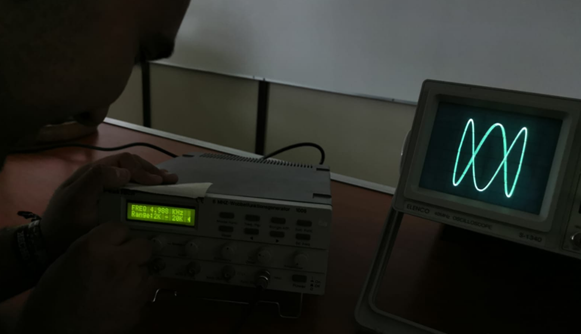
\includegraphics[width=4cm,height=5cm]{Imagenes/5.png}
	\captionof{figure}{Valor del generador proyectando la señal.}
	\label{fig:5}
\end{center}

\textbf{Señal 6}\\
\begin{center}
    
$\frac{3\omega_{1}}{2\omega_{2}}=\frac{15.030 Hz}{10.69 Hz}$\\
\end{center}
Con esta señal seguimos con la frecuencia base de 5 KHz, y ampliamos la frecuencia 1 al triple, que en un valor teórico será igual a 15 KHz y la segunda señal la ampliamos al doble que en valor teórico sería igual a 10 KHz. Dándonos como resultado a nuestra percepción una canasta. (Figura 6)
\begin{center}
	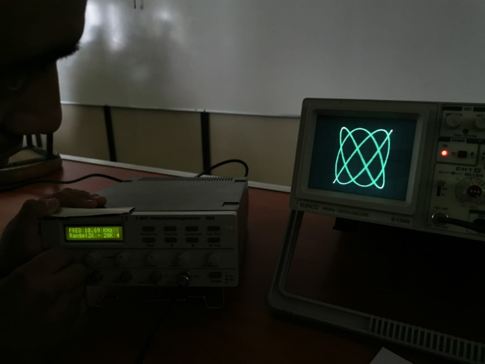
\includegraphics[width=4cm,height=5cm]{Imagenes/6.png}
	\captionof{figure}{Osciloscopio que proyecta una “canasta”, cuando una frecuencia esta triplicada y la otra esta duplicada.}
	\label{fig:6}
\end{center}


\textbf{Señal 7}\\
\begin{center}
    
$\frac{3\omega_{1}}{4\omega_{2}}=\frac{15.030 KHz}{20.57 KHz}$\\
\end{center}
Para esta señal continuamos con la misma frecuencia en el generador de señales 1, pero le sumamos al otro generador 5 KHZ más, que en un valor teórico nos daría como resultado 20 KHz, y posterior a eso logramos visualizar una figura peculiar pero dentro del intervalo de imágenes que buscábamos encontrar. (Figura 7)\\
\begin{center}
	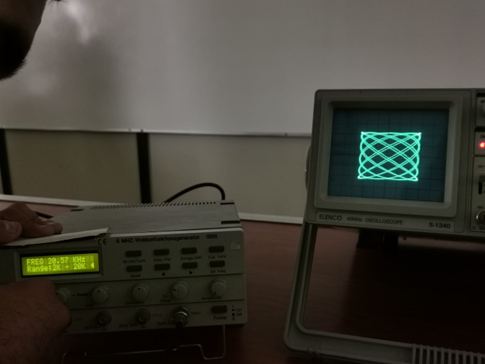
\includegraphics[width=4cm,height=5cm]{Imagenes/7.png}
	\captionof{figure}{Osciloscopio que nos muestra una señal a diferentes señales sobrepuestas.}
	\label{fig:7}
\end{center}
\textbf{Señal 8}\\
\begin{center}
    
$\frac{5\omega_{1}}{4\omega_{2}}=\frac{25.01 KHz}{20.69 KHz}$\\
\end{center}
Basándonos en que nuestra frecuencia base es de 5KHz, hicimos aritmética de preescolar para determinar a qué frecuencias nos arrojaría una imagen nuestro osciloscopio y en un valor teórico la frecuencia 1 quedaría de 25 KHZ y la frecuencia 2 quedaría de 20 KHZ. (Figura 8)\\
\begin{center}
	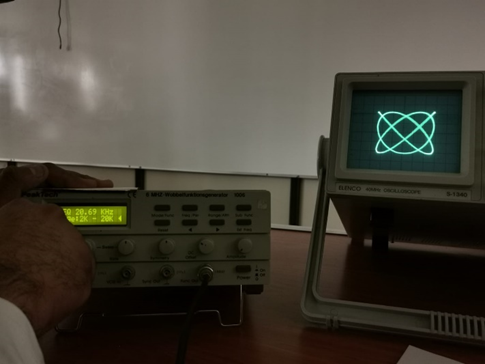
\includegraphics[width=4cm,height=5cm]{Imagenes/8.png}
	\captionof{figure}{Osciloscopio que nos muestra a nuestra interpretación un corazón, con dos anillos rodeándolo.}
	\label{fig:8}
\end{center}

\textbf{Señal 9}\\
\begin{center}
    
$\frac{\omega_{1}}{5\omega_{2}}=\frac{5 KHz}{25 KHz}$\\
\end{center}
Aquí principalmente seguimos con lo que propusimos desde la señal 4, ya que mantuvimos al generador 1 en 5KHz y en un valor teórico a la segunda onda la dejamos con 25 KHz, dándonos una imagen extrañamente estática, y desde cierta perspectiva en un eje diferente (eje “y”) proyectada. (Figura 9)
\begin{center}
	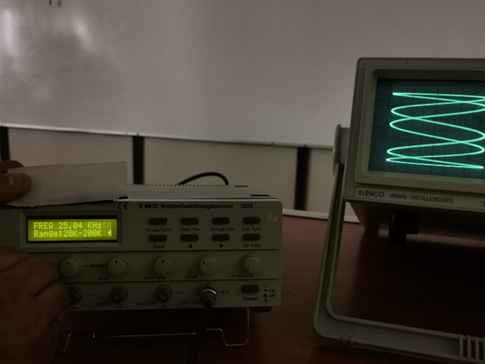
\includegraphics[width=4cm,height=5cm]{Imagenes/9.png}
	\captionof{figure}{Osciloscopio proyectando lo que a nuestra consideración es una señal normal proyectada en el eje de las “y”.}
	\label{fig:9}
\end{center}

\textbf{Señal 10}\\
\begin{center}
    
$\frac{5\omega_1}{\omega_{2}}=\frac{25.01 KHz}{4.883 KHz}$\\
\end{center}
Con los criterios anteriores de mantener una frecuencia base de 5KHz, realizamos una nueva señal pero invertimos los valores en comparación al caso anterior, por lo que la frecuencia 1 paso a ser igual a cinco veces más grande que la frecuencia 2, dándonos una valor teórico de Frecuencia 1 siendo igual a 25 KHz y la Frecuencia 2 siendo igual a 5 KHz. (Figura 10)

\begin{center}
	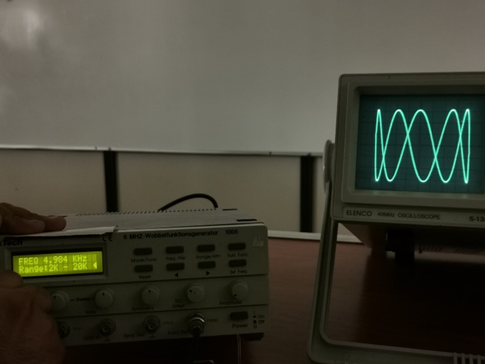
\includegraphics[width=4cm,height=5cm]{Imagenes/11.png}
	\captionof{figure}{Osciloscopio proyectando una corona en una orientación con respecto al eje de las “x”.}
	\label{fig:10}
\end{center}

\textbf{Resultados}
Datos tabulados del experimento 

\begin{center}
	\begin{adjustbox}{width=270pt}
		\begin{tabular}{|c|c|c|c|}
			\hline
			Caso  &Frecuencia $\nu_1 [Hz]$ & Frecuencia $\nu_2 [Hz]$ &Figura \\
			\hline
			$\frac{\omega_1}{\omega_2}$ &21.05 &21.05 & Figura 1 \\
			\hline
			$\frac{\omega_1}{2\omega_2}$ & 10.15&20.29 & Figura 2 \\
			\hline
			$\frac{2\omega_1}{\omega_2}$ &21.05 &10.03 & Figura 3 \\
			\hline
			$\frac{\omega_1}{3\omega_2}$ &5.113 &14.49 & Figura 4\\
			\hline
			$\frac{3\omega_1}{\omega_2}$ &15.030 & 4.988& Figura 5 \\
			\hline
            $\frac{3\omega_1}{2\omega_2}$ &15.030 &10.69 & Figura 6 \\
			\hline
            $\frac{3\omega_1}{2\omega_2}$ & 15.030& 20.57& Figura 7 \\
			\hline
            $\frac{5\omega_1}{4\omega_2}$ & 25.01& 20.69& Figura 8 \\
			\hline
            $\frac{\omega_1}{5\omega_2}$ & 5.11& 25.04& Figura 9 \\
			\hline
            $\frac{5\omega_1}{\omega_2}$ &25.01 &4.883 & Figura 10 \\
			\hline
		\end{tabular}
	\end{adjustbox}
\end{center}

Durante el desarrollo del experimento tuvimos muchas dificultades al tratar de calibrar la maquina por la gran cantidad de oscilaciones de nuestras señales,  con paciencia logramos una imagen más congruente, con las diferentes señales pudimos concluir que con cada señal sobrepuesta con diferente frecuencia cambia mucho o hasta se pueden repetir las figuras que están proyectadas en el osciloscopio tabulando todos los valores observando cada fenómeno presentado. 






\section{Conclusiones.}
\subsection{Hernández Huerta Jose Emilio.}
Por temas tecnicos personales no pude estar presente en la practica pero al transpasar el reporte a latex me doy cuenta que de cierta forma las frecuencias guardan cierta proporcionalidad cuando se trata de figuras geometricamente sem-paralelas o por decirlo de otra forma simetricas en las figuras en las que más "disparejas" noto una difefrencia mayor entre sus frecuencias por ejemplo la fiferencia de la figura 10 es aproximadamente 20Hz mientras que en las primeras son nulas o algo mas proporcionales.
\subsection{Hernández Sanluis Danna Estefany.}
En esta práctica de superposición de ondas es fundamental para explicar y predecir diversos fenómenos en física y tiene aplicaciones importantes en muchas áreas, incluyendo la tecnología de comunicaciones, la óptica y la acústica , al realizar la práctica vimos que al disminuir la frecuencia de un componente y alterar la frecuencia en otro , llegan a formar diferentes ondas y en ellas se aprecian diferentes figuras , hasta incluso se forma una cortina de ondas y se seguirán apreciando varias varias figuras conforme nosotros modifiquemos las frecuencias de ambos dispositivos .
\subsection{Nataly Bejarano Garduño.}
En el desarrollo de esta practica se logro hayar señales analogicas con el oscilador, a la vez observamos las frecuencias de las ondas lo cual hace que las ondas formen ciertas formas peculiares y llamativas, ya que entre mas frecuencia se tenga en el sistema mas movimiento tendra la onda en cuestión, lo cual tambie nos permitio ver la teoria de la superpoción de ondas el cual consiste en que la onda resultante de la interracción entre dos ondas, y esto se ve cuando dos señales en el oscilador intervienen entre ellas.
\subsection{Mojica Reyes Rogelio.}
En el desarrollo de esta práctica observamos el comportamiento de dos fenómenos, el primero de ellos como se comportan dos ondas sobrepuestas en un plano común y como inducir una con otra de manera natural para generar en estos casos diferentes tipos de formas o comportamientos. Y el otro fenómeno que observamos es como mejoramos con el dominio de instrumentos (osciloscopio y generador de señales) para provocar comportamientos y fenómenos que son de utilidad para el uso, observación y análisis de ondas (en estos casos del experimento específicamente, pero que también pueden son de gran utilidad en nuestra vida como ingenieros).
\subsection*{Morlan Juárez Bruno Tonatiuh.}
En este experimento tuve un mayor aprendizaje al usar la herramienta utilizada dentro del experimento, el control de las señales obtenidas por una frecuencia especifica es el mejor método para manipular este tipo de máquinas y lo que son capaces de hacer, también para entender mejor el fenómeno físico desde lo practico hasta lo visual. 
\subsection*{Santos Marañón María Renée.}
Cuando dos ondas se encuentran en un punto o una región del espacio, el resultado es una nueva onda cuya perturbación es la suma de las perturbaciones de las dos ondas originales. A continuación consideramos la superposición e interferencia de ondas armónicas. Se denomina interferencia al resultado de la superposición de dos o más ondas armónicas.  La onda resultante tiene una amplitud diferente, pero la misma frecuencia y 
longitud de onda que las componentes.Si la diferencia de fase es cero, se dice que las ondas están en fase y la
amplitud de la resultante es el doble de la amplitud original.
Si la diferencia de fase es cercana a 180°, la amplitud resultante es casi cero. La onda puede cambiar también de forma si cede energía mecánica al 
medio cuando se presentan fuerzas disipativas (que dependen en general 
de la velocidad).


\end{multicols}

\end{document}
